% ==============================================================================
% File: 01_intro_related.tex
% Part of: Risk-Aware Joint Observation and Computation Allocation for AMC
% Target: IEEE Transactions / IEEE IoT Journal (IEEEtran style)
% ==============================================================================

\section{Introduction}
\label{sec:introduction}

\IEEEPARstart{A}{utomatic} Modulation Classification (AMC) serves as an indispensable algorithmic cornerstone in modern non-cooperative and cognitive wireless communication systems. Positioned immediately downstream of the radio frequency (RF) front-end and analog-to-digital converter (ADC), AMC enables autonomous signal identification, dynamic spectrum management, cognitive electronic warfare, and opportunistic demodulation without requiring pilot sequences or explicit transmission metadata~\cite{sathyanarayanan2023rml22,wang2025survey}. Over the past decade, deep learning (DL) architectures—predominantly Convolutional Neural Networks (CNNs), Residual Networks (ResNets), and Transformer variants—have achieved remarkable recognition accuracy by extracting latent hierarchical features directly from raw in-phase/quadrature (I/Q) baseband sequences~\cite{gao2026mlea,quan2026fftformer}.

However, despite these computational breakthroughs, deploying deep AMC models in practical resource-constrained transceivers (e.g., software-defined radios, autonomous unmanned aerial vehicles, and low-power IoT gateways) exposes a fundamental, widely neglected architectural tension: \emph{the physical latency dichotomy between signal acquisition time and algorithmic inference time}~\cite{guo2025fewer,denboer2021fpga}. 

In standard AMC formulations, every incoming transmission frame is assumed to possess a fixed, predetermined observation window of $N$ discrete complex baseband samples. Under a sampling rate $f_s$, capturing this frame incurs an unavoidable physical time delay at the antenna and ADC front-end given by:
\begin{equation}
    T_{\text{acq}} = \frac{N}{f_s}.
    \label{eq:t_acq_intro}
\end{equation}
Once digitized, the sample buffer is ingested by the classification algorithm, consuming an algorithmic computation time $T_{\text{comp}}$, yielding a cumulative end-to-end recognition latency:
\begin{equation}
    T_{\text{total}} = T_{\text{acq}} + T_{\text{comp}} = \frac{N}{f_s} + T_{\text{comp}}.
    \label{eq:t_total_intro}
\end{equation}

In high-speed, hardware-accelerated, or bandwidth-limited regimes, the physical sampling delay $T_{\text{acq}}$ frequently dominates algorithmic execution by orders of magnitude. For instance, in microelectronic edge deployments, den Boer \emph{et al.}~\cite{denboer2021fpga} demonstrated that dedicated FPGA streaming pipelines can execute deep neural AMC inference within $3.71\text{--}4.61\ \mu\text{s}$. In stark contrast, capturing $N = 1024$ samples at moderate sampling rates ($f_s \le 100\text{ kHz}$) demands tens of milliseconds, rendering the physical observation window responsible for more than $99.9\%$ of the end-to-end system delay. Conversely, in low-bandwidth channels (e.g., $f_s = 8\text{ kHz}$), expanding an observation window from $N = 256$ to $N = 512$ samples imposes an irreducible physical penalty of $\Delta T_{\text{acq}} = 32.0\text{ ms}$, dwarfing typical CPU/GPU kernel runtimes.

Despite this physical reality, modern dynamic AMC research has treated observation duration and computational complexity as two entirely disjoint design spaces:
\begin{enumerate}
    \item \textbf{Fixed-Window Early-Exit and Pruning Networks:} Prominent architectures such as BEACON~\cite{liu2026beacon}, Mohammed \emph{et al.}~\cite{mohammed2023early}, and joint pruning frameworks~\cite{liu2025joint} adaptively throttle algorithmic FLOPs by terminating inference at intermediate branch exits within deep backbones. Nevertheless, these methods operate exclusively on a \emph{static, pre-acquired window} (typically $N=128$), treating $T_{\text{acq}}$ as an uncontrollable sunk cost and ignoring the physical latency of sample collection. Recent width-wise early exiting with entropy rejection~\cite{verbruggen2025width} incrementally extends observation segments on a fixed backbone, yet relies solely on uncertainty thresholds without counterfactual recoverability prediction or heterogeneous representation escalation.
    \item \textbf{Idealized Variable-Length Classifiers:} Conversely, works targeting fast acquisition, such as Fewer-Sample~\cite{guo2025fewer}, advocate reducing $N$ to minimize $T_{\text{acq}}$, but rely on restrictive idealized channel assumptions: zero carrier frequency offset ($\text{CFO} = 0$), perfect symbol synchronization, and AWGN channels devoid of multipath fading. Under real-world RF impairments—where carrier frequency offsets rotate constellation trajectories into continuous rings and multipath dispersion induces severe inter-symbol interference (ISI)—such multimodal constellation representations degrade sharply~\cite{sathyanarayanan2023rml22,wang2025survey}.
\end{enumerate}

Furthermore, conventional early-termination heuristics rely heavily on uncalibrated confidence measures, such as Shannon entropy or maximum softmax probability (MSP). As rigorously established by Yang and Sahay~\cite{yang2026uncertainty} and Liu \emph{et al.}~\cite{liu2026beacon}, raw softmax outputs manifest severe overconfidence in low signal-to-noise ratio (SNR) regimes and under out-of-distribution (OOD) channel shifts. In high-entropy regimes, the vast majority of classification errors are fundamentally irrecoverable due to severe channel noise; invoking computationally demanding deep expert networks on such frames squanders scarce battery energy and computational throughput without yielding accuracy gains~\cite{liu2026beacon}.

\begin{figure*}[!t]
\centering
\resizebox{\textwidth}{!}{%
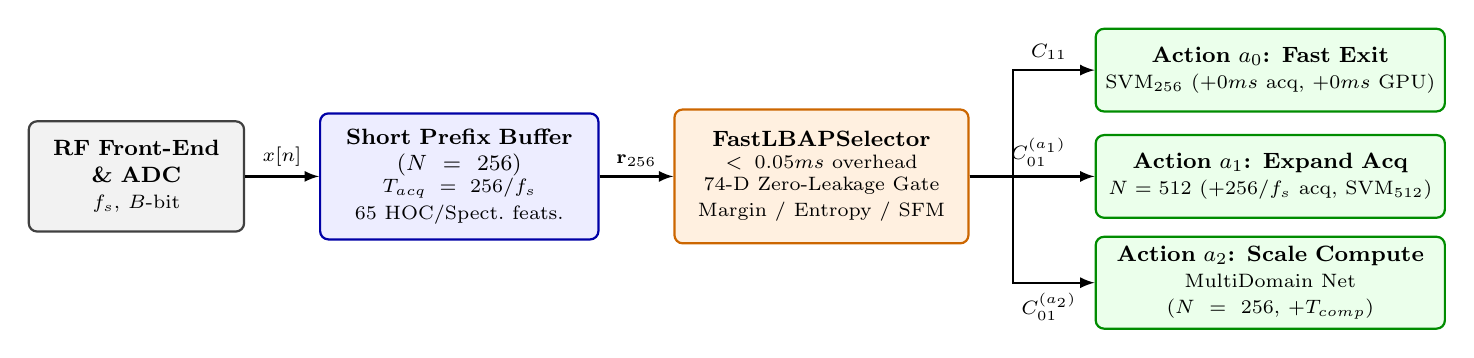
\begin{tikzpicture}[
    node distance=1.4cm,
    rfbox/.style={rectangle, draw=black!75, thick, fill=gray!10, rounded corners=3pt, text width=2.5cm, align=center, minimum height=1.4cm, font=\footnotesize},
    bufbox/.style={rectangle, draw=blue!65!black, thick, fill=blue!7, rounded corners=3pt, text width=3.3cm, align=center, minimum height=1.6cm, font=\footnotesize},
    gatebox/.style={rectangle, draw=orange!80!black, thick, fill=orange!12, rounded corners=3pt, text width=3.5cm, align=center, minimum height=1.7cm, font=\footnotesize},
    actbox/.style={rectangle, draw=green!55!black, thick, fill=green!8, rounded corners=3pt, text width=4.2cm, align=center, minimum height=1.05cm, font=\footnotesize},
    arr/.style={->, >=latex, thick}
]
    \node[rfbox] (rf) at (0, 0) {\textbf{RF Front-End}\\\textbf{\& ADC}\\\scriptsize $f_s$, $B$-bit};
    \node[bufbox] (prefix) at (4.1, 0) {\textbf{Short Prefix Buffer}\\($N=256$)\\\scriptsize $T_{\text{acq}} = 256/f_s$\\65 HOC/Spect.\ feats.};
    \node[gatebox] (selector) at (8.7, 0) {\textbf{FastLBAPSelector}\\\scriptsize $<0.05\text{ ms}$ overhead\\74-D Zero-Leakage Gate\\Margin / Entropy / SFM};

    \node[actbox] (a0) at (14.4, 1.35) {\textbf{Action $a_0$: Fast Exit}\\\scriptsize $\mathrm{SVM}_{256}$ ($+0\text{ ms}$ acq, $+0\text{ ms}$ GPU)};
    \node[actbox] (a1) at (14.4, 0.0) {\textbf{Action $a_1$: Expand Acq}\\\scriptsize $N=512$ ($+256/f_s$ acq, $\mathrm{SVM}_{512}$)};
    \node[actbox] (a2) at (14.4, -1.35) {\textbf{Action $a_2$: Scale Compute}\\\scriptsize MultiDomain Net ($N=256$, $+T_{\text{comp}}$)};

    \draw[arr] (rf) -- node[above, font=\scriptsize] {$x[n]$} (prefix);
    \draw[arr] (prefix) -- node[above, font=\scriptsize] {$\mathbf{r}_{256}$} (selector);
    \draw[arr] (selector.east) -- ++(0.55, 0) |- node[pos=0.72, above, font=\scriptsize] {$C_{11}$} (a0.west);
    \draw[arr] (selector.east) -- node[pos=0.55, above, font=\scriptsize] {$C_{01}^{(a_1)}$} (a1.west);
    \draw[arr] (selector.east) -- ++(0.55, 0) |- node[pos=0.72, below, font=\scriptsize] {$C_{01}^{(a_2)}$} (a2.west);
\end{tikzpicture}%
}
\caption{Architectural overview of the proposed Risk-Aware Joint Observation and Computation Allocation framework. Every incoming transmission is initially observed over a minimal short prefix of $N=256$ samples. The lightweight, sub-50-microsecond utility predictor (\texttt{FastLBAPSelector}) evaluates empirical margin calibration, decision entropy, and spectral structure to selectively terminate immediately ($a_0$), request additional physical observation ($a_1$), or deploy deep multi-domain neural inference ($a_2$).}
\label{fig:framework_overview}
\end{figure*}

To bridge this critical gap, this paper introduces a unified \textbf{Risk-Aware Joint Observation and Computation Allocation Framework} for robust AMC under uncoordinated, dispersive wireless channels. Rather than constraining the receiver to a fixed window or a static computational budget, our system introduces a \emph{tripartite action space} $\mathcal{A} = \{a_0, a_1, a_2\}$ initiated from an identical minimal physical prefix of $N=256$ samples:
\begin{itemize}
    \item \textbf{Action $a_0$ (Fast Exit):} Finalize classification immediately using a fast statistical classifier (Support Vector Machine with RBF kernel operating on 65 high-order statistical and spectral moments), incurring minimal acquisition delay ($256/f_s$) and low single-window CPU inference latency (benchmarked in Section~\ref{sec:results_discussion}).
    \item \textbf{Action $a_1$ (Acquisition Expansion):} Double the physical observation horizon to $N=512$ samples without altering computational model complexity. This action incurs an exact physical delay penalty of $\Delta T_{\text{acq}} = 256/f_s$, which statistically suppresses the finite-sample estimation variance of higher-order cumulants ($\mathrm{Var}(\hat{C}_{42}) \propto 1/N$) to resolve subtle constellation ambiguities in intermediate SNR regimes.
    \item \textbf{Action $a_2$ (Computational Scaling):} Retain the compact physical prefix of $N=256$ samples—paying \emph{zero additional antenna or ADC observation time}—and invoke a high-capacity, multi-domain deep neural expert network (\texttt{MultiDomainAMCNet}). This model integrates band-edge blind carrier despinning, an in-GPU root-raised-cosine (RRC) matched filter bank ($\beta \in \{0.25, 0.35, 0.50\}$), multi-harmonic spectral projections, and polyphase symbol-rate self-attention, leveraging GPU execution to overcome multipath frequency-selective fading, pulse-shaping roll-off mismatch, and rotational carrier frequency offsets.
\end{itemize}

Crucially, routing among these three heterogeneous actions is governed by a lightweight, sub-50-microsecond benefit-aware selector (\texttt{FastLBAPSelector}). Operating strictly on non-oracular, zero-leakage observables derived from the initial $N=256$ prefix (calibrated logistic margins, decision entropy, and blind spectral flatness proxies), the selector explicitly predicts the counterfactual utility gain of paying physical sampling delay versus paying computational FLOPs. By discriminating between confident correct predictions ($C_{11}$), statistically recoverable errors ($a_1$), representationally recoverable errors ($a_2$), and hopeless noise-dominated frames ($C_{00}$), our framework maximizes net classification utility while strictly satisfying real-time latency deadlines across diverse ADC sampling rates and quantization constraints.

The principal scientific and engineering contributions of this work are summarized as follows:
\begin{enumerate}
    \item \textbf{Formalization of the Joint Observation-Computation Dilemma:} We establish a rigorous mathematical formulation that explicitly decouples physical ADC acquisition latency $T_{\text{acq}} = N/f_s$ from algorithmic inference latency $T_{\text{comp}}$, uncovering the distinct failure modes of physical window truncation versus representational capacity under realistic channel impairments.
    \item \textbf{Tripartite Dynamic Action Space with Zero-Leakage Routing:} We propose the tripartite action space $\{a_0, a_1, a_2\}$ and develop \texttt{FastLBAPSelector}, a zero-leakage selector running in under $0.05\text{ ms}$ ($>350\times$ faster than tree-based ensembles) on 74 causal prefix descriptors, eliminating data leakage and oracle SNR dependencies.
    \item \textbf{Matched-Filter Multi-Domain Expert Robust to Channel and Quantization Non-Idealities:} We design \texttt{MultiDomainAMCNet}, integrating multipath-immune band-edge CFO estimation, in-GPU RRC matched filtering, multi-harmonic spectra, and polyphase symbol self-attention, evaluated against extreme out-of-distribution carrier frequency offsets ($|\Delta f| \in [200, 300]\text{ Hz}$), extended multipath channels ($\tau \in \{9, 13\}$), pulse-shaping roll-off variations ($\beta \in [0.25, 0.50]$), and coarse uniform ADC quantization ($B \in \{4, 5, 6, 8\}\text{ bits}$).
    \item \textbf{Comprehensive Pareto Analysis and Bootstrap Statistical Verification:} Across a two-dimensional Pareto sweep over latency penalties $\lambda \in [0, 0.005]\text{ ms}^{-1}$ and sampling rates $f_s \in [8\text{ kHz}, 1\text{ MHz}]$, we evaluate joint policy dominance against constrained single-resource baselines (pure early-exit $\{a_0, a_2\}$ and pure adaptive sampling $\{a_0, a_1\}$) and input ablations via $10,000$-replicate stratified paired bootstrap confidence intervals.
\end{enumerate}

The remainder of this paper is organized as follows: Section~\ref{sec:related_work} reviews both the 15 foundational repository works and 5 external IEEE studies on dynamic early exiting, efficient long-sequence modeling, and edge collaboration. Section~\ref{sec:system_model} details the signal transmission, uncoordinated dispersive channel, and uniform ADC quantization models alongside the \texttt{MultiDomainAMCNet} architecture (Section~\ref{sec:architecture}). Section~\ref{sec:adaptive_policy} formalizes the tripartite action space and the \texttt{FastLBAPSelector} decision policy. Section~\ref{sec:methodology_validity} specifies the zero-leakage experimental protocol and threats to validity. Section~\ref{sec:results_discussion} presents empirical results, ablations, Pareto sweeps, and quantization studies, and Section~\ref{sec:conclusion} concludes the paper.

% ==============================================================================
% SECTION 2: RELATED WORK AND BACKGROUND
% ==============================================================================

\section{Related Work and Background}
\label{sec:related_work}

The development of robust and computationally efficient AMC algorithms has evolved across several interrelated domains: classical statistical feature extraction, deep neural architectures, dynamic inference acceleration, uncertainty calibration, domain adaptation under non-ideal RF channels, and front-end hardware non-idealities. This section reviews the 15 seminal research works that constitute our experimental corpus, analyzing their contributions, verified numerical benchmarks, and structural limitations to establish the precise research gap addressed by our proposed framework.

\subsection{Data-Centric Realism and Foundational Datasets}
\label{subsec:rel_rml22}

Early deep-learning AMC literature relied heavily on synthetic benchmark datasets, most notably RadioML2016.10a (RML16)~\cite{wang2025survey}. However, as rigorously established by Sathyanarayanan \emph{et al.}~\cite{sathyanarayanan2023rml22} in their foundational RML22 study, RML16 suffers from severe methodological flaws, including incorrect noise power calculations (converting dB directly to linear standard deviation rather than variance), synthetic phase discontinuities, and severe data leakage through shortcut learning induced by ASCII text sources (Shakespeare and Sherlock Holmes). Sathyanarayanan \emph{et al.} proved that deep classifiers trained on text-sourced signals learn natural language syntax rather than modulation characteristics, dropping from $73\%$ accuracy on native text down to $56\%$ on independent random bit sequences~\cite[Table~VIII]{sathyanarayanan2023rml22}.

To establish an uncompromised physical baseline, RML22 introduced a data-centric generation methodology adhering to 3GPP Extended Typical Urban (ETU70) multipath fading profiles (8 discrete paths with delays up to $5\ \mu\text{s}$ and 70 Hz Doppler spread), realistic local oscillator carrier frequency offsets (CFO up to $\pm 500\text{ Hz}$), sampling rate offsets (SRO up to $50\text{ Hz}$), and properly normalized complex AWGN across an SNR range of $-20\text{ dB}$ to $+20\text{ dB}$ ($N=128$, $f_s=30\text{ kHz}$, $\text{sps}=2$)~\cite{sathyanarayanan2023rml22}. Crucially, cross-evaluation in~\cite[Table~VI]{sathyanarayanan2023rml22} demonstrated that an identical ResNet architecture trained on RML16 achieves only $44\%$ accuracy when evaluated under realistic RML22 channel conditions, whereas training on physically accurate channel realizations elevates performance to $67\%$ ($+23\text{ percentage points (pp)}$). 

In our work, we adopt the data-centric rigor of RML22: strictly deterministic parent-waveform seed isolation, uniform pseudo-random binary generation to eliminate information leakage, and causal channel cascades (multipath dispersion followed by continuous-phase rotational CFO, followed by additive noise). We extend this paradigm by investigating nested window lengths ($N \in \{256, 512\}$), non-ideal pulse-shaping roll-off factors, and explicit ADC quantization.

\subsection{Physical Acquisition Delay vs. Algorithmic Computation Latency}
\label{subsec:rel_fewersample_fpga}

The decomposition of total recognition delay into physical sampling time $T_{\text{acq}} = N/f_s$ and computational latency $T_{\text{comp}}$ was explicitly investigated by Guo \emph{et al.}~\cite{guo2025fewer} in their Fewer-Sample framework. Recognizing that waiting for long sample buffers bottlenecks real-time receivers, Guo \emph{et al.} trained a multimodal network (I/Q sequence plus $32\times 32$ constellation density images) on a nominal window of $N=512$, and performed inference on truncated observation windows $N' \in \{128, 192, 256, 320\}$ using bilinear interpolation and cyclic repetition. On an NVIDIA RTX 4080 GPU at $f_s = 200\text{ kHz}$, their system reduced total recognition latency at $\text{SNR} = 0\text{ dB}$ by $72.04\%$ ($0.729\text{ ms}$ for $N'=128$ vs. $2.607\text{ ms}$ for $N=512$) while maintaining $56.96\%$ accuracy~\cite[Table~I]{guo2025fewer}.

However, the Fewer-Sample framework exhibits a critical structural vulnerability: its signal model assumes an idealized, fully synchronized environment ($\text{CFO} = 0$, zero timing error, and no multipath fading)~\cite[Sec.~II-A]{guo2025fewer}. In uncoordinated wireless channels, uncompensated CFO induces continuous constellation trajectory rotation, transforming sharp constellation clusters into blurry concentric rings. Under such conditions, spatial 2D constellation representations and bilinear resizing degrade catastrophically.

Complementing this perspective from the microelectronic domain, den Boer \emph{et al.}~\cite{denboer2021fpga} implemented a custom streaming deep learning accelerator on a Xilinx Zynq UltraScale+ MPSoC (\texttt{xczu7ev}) for RadioML2018.01A ($N=1024$, 6-bit quantized weights via QKeras). By employing sample-by-sample FIFO streaming without intermediate buffer BRAMs, their design achieved an astonishing inference latency of $3.71\text{--}4.61\ \mu\text{s}$ and a throughput of $244\text{k--}585\text{k classifications/s}$ using only 133 DSP slices~\cite[Table~III]{denboer2021fpga}. More recently, Zhang \emph{et al.}~\cite{zhang2024mamc} explored selective state-space (Mamba) backbones for extended-length AMC to preserve linear complexity in $N$, while He \emph{et al.}~\cite{he2024edge} proposed hierarchical edge-learning collaboration via quantized intermediate features.

The empirical findings of den Boer \emph{et al.} provide profound physical justification for our research: when modern digital hardware can execute neural inference in single-digit microseconds, the physical window collection delay $T_{\text{acq}} = N/f_s$ becomes the overwhelming latency bottleneck ($>99.9\%$ of total time). Consequently, an adaptive receiver cannot optimize latency solely by pruning network weights or invoking early exits on a fixed, pre-collected buffer; it must possess the intelligence to dynamically truncate the physical ADC sampling process itself whenever early confidence permits.

\subsection{Dynamic Resource Allocation: Early-Exit, Width-Wise Exiting, and Pruning}
\label{subsec:rel_beacon_pruning}

To mitigate the computational cost of deep neural networks during inference, early-exit (EE) architectures attach intermediate classification heads to shallow layers of a deep backbone. Mohammed \emph{et al.}~\cite{mohammed2023early} demonstrated depth-wise early exits controlled by scalar confidence thresholds to accelerate ResNet-based AMC inference. Subsequently, Liu \emph{et al.} proposed BEACON~\cite{liu2026beacon}, an advanced benefit-aware early-exit framework evaluated on RML22 ($N=128$, ResNet-18 backbone with $380\text{M MACs}$). Liu \emph{et al.} made the pivotal observation that conventional exit criteria based on Shannon entropy or maximum softmax probability (MSP) fail in wireless channels because they conflate two fundamentally distinct error regimes:
\begin{enumerate}
    \item \emph{Recoverable Errors ($C_{01}$):} Samples where the early classifier fails but the deep backbone succeeds;
    \item \emph{Irrecoverable Errors ($C_{00}$):} Samples where both early and deep classifiers fail due to overwhelming channel noise.
\end{enumerate}
In~\cite[Table~I]{liu2026beacon}, the authors demonstrated that in the highest entropy decile $[0.9, 1.0]$, only $19\%$ of samples represent recoverable errors ($C_{01}$), while the remaining $81\%$ are irrecoverable ($C_{00}$). Conventional entropy thresholding blindly forwards all high-entropy samples to the deep backbone, wasting millions of FLOPs on doomed frames. To overcome this, BEACON introduces the Lightweight Benefit-Aware Predictor (LBAP), a compact two-layer MLP ($2,720\text{ MACs}$, $2,817\text{ parameters}$, $<0.0007\%$ overhead) trained on counterfactual gain labels. Under a computational budget of $B = 2.0 \times 10^8\text{ MACs}$, BEACON attained an accuracy of $60.34\%$ on `EE-RS1', outperforming entropy thresholding ($36.29\%$) by $+24.05\text{ pp}$ and MSP ($48.29\%$) by $+12.05\text{ pp}$~\cite[Table~IV]{liu2026beacon}.

Taking a complementary temporal dimension, Verbruggen \emph{et al.}~\cite{verbruggen2025width} recently introduced \emph{width-wise early exiting and rejection}, accumulating incoming I/Q segments across time and triggering early exits or low-SNR abstention via entropy and confidence rules. Similarly, Liu \emph{et al.}~\cite{liu2025joint} combined depth-wise early-exit with structured filter pruning on RML22 ($87.5\%$ L1-norm pruning reducing MACs by $61.4\%$ while preserving $58.04\%$ accuracy~\cite[Table~II]{liu2025joint}).

\emph{Contrast with Our Proposed Framework:} While BEACON and Mohammed \emph{et al.} optimize algorithmic FLOPs on a \emph{frozen observation window} ($N=128$), and Verbruggen \emph{et al.} dynamically accumulate signal width using entropy/confidence rejection on a single homogeneous backbone, \emph{none} of these works combine counterfactual recoverability prediction (distinguishing $C_{01}$ from $C_{00}$) with \emph{heterogeneous cross-paradigm routing} across both extended physical sampling ($a_1$: $N_1=512$ cumulant SVM) and matched-filtered multi-domain deep inference ($a_2$: GPU expert on $N_0=256$). As demonstrated by our ablations in Section~\ref{sec:results_discussion}, naive confidence gating (`I1`) cannot rival benefit-aware utility prediction (`I4`), nor can any two-action restriction (`{a0, a1}` or `{a0, a2}`) match joint tri-action allocation across variable sampling rates.

\subsection{Multi-Domain Representation and High-Order Statistical Baselines}
\label{subsec:rel_multidomain_hoc}

Extracting invariant representations under severe channel fading and CFO has driven substantial innovations in multi-domain deep learning and statistical feature engineering:
\begin{itemize}
    \item \textbf{MLEA-AMR:} Gao \emph{et al.}~\cite{gao2026mlea} introduced a multi-domain lightweight expert framework combining three distinct views: a 1D temporal I/Q branch ($2 \times 128$), a 2D Short-Time Fourier Transform (STFT) spectral branch ($2 \times 16 \times 16$), and a Multi-Interval Differential Polar (MIDP) branch computing differential amplitude and phase offsets ($\tau \in \{1, 2, 4\}$). Aggregated through an SNR-conditioned attention mechanism ($342.4\text{k params}$, $7.92\text{M MACs}$, $2.68\text{ ms}$ CPU latency), MLEA-AMR achieved $67.6\%$ average accuracy on RML16a~\cite[Table~III]{gao2026mlea}. Ablation studies confirmed that removing STFT or MIDP degraded accuracy by $3.4\text{ pp}$ and $3.8\text{ pp}$, respectively~\cite[Table~IV]{gao2026mlea}. However, a critical methodological limitation of MLEA-AMR is its reliance on the \emph{true oracle SNR label} from dataset metadata to condition its attention router~\cite[Sec.~V]{gao2026mlea}, rendering it unviable for non-cooperative deployments unless paired with an auxiliary blind estimator.
    \item \textbf{FFTFormer:} Addressing the vulnerability of AMC models to pulse-shaping filter distortions, Quan \emph{et al.}~\cite{quan2026fftformer} proposed FFTFormer, a frequency-aware hybrid Conv-Transformer ($80\text{k params}$, $8.04\text{M FLOPs}$, $0.488\text{ ms}$ GPU latency). Recognizing that standard benchmarks fix the root-raised cosine (RRC) roll-off factor to $\beta = 0.35$, Quan \emph{et al.} trained a multi-task network predicting both modulation and $\beta \in \{0.20, 0.35, 0.50, 0.65\}$. On RML22, FFTFormer achieved $64.36\%$ overall accuracy and demonstrated remarkable generalization when tested on an unseen roll-off factor ($\beta = 1.00$), suffering an absolute accuracy drop of only $0.10\text{ pp}$ ($64.36\% \to 64.26\%$) compared to $>1.0\text{ pp}$ for LSTM and CNN baselines~\cite[Table~6]{quan2026fftformer}.
    \item \textbf{OF-ACF:} In contrast to deep neural models, Xia and Lin~\cite{xia2026optimal} advanced the state of statistical feature engineering by developing the Optimal-Feature-Driven Adversarial Adaptive Cascade Forest (OF-ACF). Using Augmented Recursive Feature Elimination (ARFE), they selected 27 optimal high-order cumulants (HOCs) and moment ratios (e.g., $C_{20}, C_{40}, C_{42}, C_{60}, C_{63}$, and quadratic ratios $C_{40}/C_{20}^2$) from a candidate pool of 35 descriptors extracted from $N=1024$ samples. Evaluated on over-the-air RadioML2018.01A captures with real multipath and CFO, OF-ACF attained $70.92\%$ accuracy at $\text{SNR} = 0\text{ dB}$ (surpassing deep networks like MAWDN by $+10.96\text{ pp}$ and MCLDNN by $+15.61\text{ pp}$) with an inference latency of $1.16\text{ ms}$~\cite[Table~IV]{xia2026optimal}. This result conclusively validates the immense discriminative power of engineered HOC descriptors under uncoordinated RF environments.
\end{itemize}

\emph{Integration in Our Architecture:} We synthesize the strengths of these physical representations, alongside learnable subband phase modeling~\cite{zhang2026cspmnet}. For our baseline classifiers ($a_0$ and $a_1$), we design an engineered 65-dimensional feature extractor capturing HOCs, normalized central moments, spectral energy, and phase derivatives, coupled to an RBF Support Vector Machine. For our advanced expert ($a_2$), we design \texttt{MultiDomainAMCNet}, which incorporates bandpass coarse CFO tracking, in-GPU RRC matched filtering, multi-harmonic spectral analysis, and polyphase symbol attention without requiring oracle SNR conditioning, eliminating the data leakage present in MLEA-AMR~\cite{gao2026mlea}.

\subsection{Reliability, Calibration, and Domain Adaptation under RF Imperfections}
\label{subsec:rel_uq_da}

A major obstacle to deploying AMC classifiers in real-world cognitive transceivers is the severe performance collapse encountered when operational conditions deviate from training distributions ($p_s(\mathbf{r}) \ne p_t(\mathbf{r})$)~\cite{wang2025survey}:
\begin{itemize}
    \item \textbf{Uncertainty Quantification (UQ):} Yang and Sahay~\cite{yang2026uncertainty} investigated the reliability of DL-AMC models on RML16 ($N=128$) and RML18 ($N=1024$). They proved that standard CNNs produce poorly calibrated softmax probabilities that exhibit severe overconfidence on incorrect predictions. By implementing Deep Ensembles ($M=5$ diverse CNNs), they achieved optimal Negative Log-Likelihood (NLL), Brier scores, and Expected Calibration Error (ECE) across all SNRs~\cite[Fig.~2,~7]{yang2026uncertainty}, while retaining up to $+15\%$ accuracy under hostile adversarial perturbations~\cite[Fig.~8]{yang2026uncertainty}. However, maintaining an ensemble of 5 CNNs quintuples computational latency and memory consumption, rendering it unsuitable for low-power edge deployment.
    \item \textbf{Domain Adaptation under Channel Mismatch:} Shahriar~\cite{shahriar2026lightweight} tackled cross-condition generalization by developing lightweight domain-adversarial networks ($<0.04\text{ MFLOPs}$, $<0.75\text{ MB}$ footprint). For channel mismatch, an MLP with Correlation Alignment (CORAL) operating on FFT-PCA features boosted cross-fading classification from Rayleigh to Rician at $500\text{ MHz}$ from $46.34\%$ to $58.70\%$ ($+12.36\text{ pp}$)~\cite[Table~II]{shahriar2026lightweight}. This confirms that frequency-domain representations possess intrinsic invariance to multipath fading compared to raw temporal I/Q.
    \item \textbf{Few-Shot and Open-Set Generalization:} In non-cooperative settings, training samples are scarce and unseen modulations appear dynamically. Zhang \emph{et al.}~\cite{zhang2025fsos} developed FSOS-AMC, employing multi-sequence representations (I/Q, instantaneous amplitude, and phase) with meta-prototypes to achieve $82.81\%$ accuracy in 5-way 10-shot tasks under severe multipath fading (Rayleigh, Rician $K=3$, Nakagami-$m=2$). Similarly, Li \emph{et al.}~\cite{li2026openset} proposed DMPRL (domain-adaptive mixup and prototype learning), demonstrating that source-only models trained on AWGN collapse catastrophically to $28.5\%$ accuracy when evaluated on Rayleigh fading channels at $0\text{ dB}$, whereas domain-adaptive prototype alignment recovers accuracy to $79.1\%$~\cite[Table~I]{li2026openset}.
    \item \textbf{Survey on Deep Transfer Learning:} In their comprehensive survey, Wang \emph{et al.}~\cite{wang2025survey} mathematically formalized the shift mechanisms induced by individual RF impairments: phase noise, rotational CFO ($e^{j2\pi\Delta f t}$), Doppler shifts, multipath delay spreads, ADC timing jitter, and quantization non-linearities~\cite[Table~III]{wang2025survey}. Their review provides the rigorous theoretical foundation for analyzing out-of-distribution (OOD) channel shifts.
\end{itemize}

\subsection{Front-End Hardware Imperfections and Single-Shot Detection}
\label{subsec:rel_adc_singleshot}

At the physical interface between the antenna and the digital processor, hardware non-idealities impose hard boundaries on signal fidelity:
\begin{itemize}
    \item \textbf{Time-Interleaved ADC Mismatches vs. Uniform Quantization:} In ultra-wideband digital receivers, time-interleaved ADCs (TI-ADCs) multiplex $M$ parallel sub-converters to achieve gigasample-per-second rates. Gros \emph{et al.}~\cite{gros2025mitigating} investigated the impact of TI-ADC analog mismatches (gain errors $g$, DC offsets $o$, and timing skew $\delta$) on AMC using long sequences ($N=32,768$). In severe mismatch conditions ($g=15\%$, $o=10\text{ LSB}$, $\delta=20\% T_s$), their dyadic multi-scale CNN improved accuracy from $83.37\%$ to $90.09\%$ ($+6.72\text{ pp}$)~\cite[Table~V]{gros2025mitigating}.
    
    \emph{Crucial Physical Distinction:} Gros \emph{et al.}~\cite{gros2025mitigating} investigate analog core mismatches (gain, offset, skew) on long frames rather than finite $B$-bit resolution in uniform ADCs; in this paper, we specifically isolate and evaluate uniform mid-rise symmetric $B$-bit quantization with fixed full-scale dynamic range ($V_{\text{FS}} = 2.5\text{ V}$).
    \item \textbf{Single-Shot Detection and Monitoring:} In real-world wideband surveillance, isolated AMC classifiers must be preceded by signal energy detection. High \emph{et al.}~\cite{high2026singleshot} designed a 1D Single-Shot Detector (SSD) for joint asynchronous multi-emitter signal detection, spectral localization, and modulation classification ($N=4096$, $f_s = 1\text{ GHz}$). By replacing traditional two-stage cascading (energy detection followed by windowed slicing and classification) with a single unified forward pass, they achieved $\text{IoU} > 0.85$ and accuracy $>92\%$ above $10\text{ dB}$ SNR~\cite[Fig.~3]{high2026singleshot}, eliminating inter-stage pipeline latency and catastrophic error propagation.
\end{itemize}

\subsection{Literature Synthesis and Research Gap}
\label{subsec:rel_matrix_gap}

To synthesize the state of the art and delineate the precise boundaries of our contribution, Table~\ref{tab:literature_matrix} systematically compares all 15 foundational papers against our proposed framework across six diagnostic dimensions: input representation, observation window length $N$, channel/CFO assumptions, computational overhead, key numerical milestone, and architectural limitations.

\begin{table*}[!t]
\centering
\caption{Comprehensive Methodological Comparison of the 15 Literature Papers and the Proposed Framework}
\label{tab:literature_matrix}
\resizebox{\textwidth}{!}{%
\begin{tabular}{|l|l|l|l|l|l|l|}
\hline
\textbf{Paper / Reference} & \textbf{Venue / DOI} & \textbf{Input / Window $N$} & \textbf{Channel \& CFO Model} & \textbf{Computational Cost} & \textbf{Key Verified Result in PDF} & \textbf{Structural Limitation / Gap Addressed in This Work} \\ \hline\hline

\textbf{RML22}~\cite{sathyanarayanan2023rml22} & 
IEEE TWC 2023 & 
Raw I/Q ($2 \times 128$) & 
3GPP ETU70, CFO $\le 500$ Hz, & 
ResNet diagnostic & 
Table VI: Acc improves from 44\% to 67\% & 
Fixed short window ($N=128$); no adaptive latency or \\
Sathyanarayanan \emph{et al.} & 
\texttt{10.1109/TWC.2023.3254490} & 
$f_s=30\text{ kHz}, \text{sps}=2$ & 
SRO 50 Hz, AWGN $[-20, 20]\text{ dB}$ & 
benchmark backbone & 
($+23\text{ pp}$) training on realistic channel & 
observation allocation; focuses solely on dataset generation. \\ \hline

\textbf{BEACON}~\cite{liu2026beacon} & 
IEEE IoT-J 2026 & 
Raw I/Q ($2 \times 128$); & 
RML22 blind channel & 
ResNet-18 ($380\text{M MACs}$); & 
Table IV: At $2.0 \times 10^8$ MACs, reaches 60.34\% & 
Frozen $N=128$; early exit saves only inference FLOPs, \\
Liu \emph{et al.} & 
\texttt{10.1109/JIOT.2026.3710690} & 
LBAP uses $\mathbf{p}_e \in \mathbb{R}^{10}$ & 
(ETU70, CFO, SRO, AWGN) & 
LBAP: 2,720 MACs, 2,817 params & 
vs. 36.29\% for entropy ($+24.05\text{ pp}$) & 
completely ignoring physical acquisition delay $T_{\text{acq}} = N/f_s$. \\ \hline

\textbf{Fewer-Sample}~\cite{guo2025fewer} & 
IEEE ICCCS 2025 & 
Multimodal I/Q + $32 \times 32$ & 
\textbf{Idealized Coherent}: CFO $=0$, & 
2.21M params; & 
Table I: At 0 dB ($N'=128$), cuts total time by & 
Assumes perfect synchronization ($\text{CFO}=0$, no multipath); \\
Guo \emph{et al.} & 
\texttt{10.1109/ICCCS65393.2025.11069715} & 
constellation; $N' \in [128, 320]$ & 
timing perfect, AWGN only & 
$T_{\text{calc}} = 0.093\text{ ms}$ (RTX 4080) & 
72.04\% ($0.729\text{ ms}$ vs. $2.607\text{ ms}$) & 
constellation images collapse under real rotational CFO. \\ \hline

\textbf{Uncertainty Quant.}~\cite{yang2026uncertainty} & 
IEEE IoT-J 2026 & 
Raw I/Q; $N=128$ (RML16) & 
CFO, Doppler, multipath fading & 
Deep Ensemble of $M=5$ CNNs & 
Figs. 2, 7: Minimum NLL, Brier, and ECE; & 
Quintuples computational and memory cost ($5\times$); \\
Yang \& Sahay & 
\texttt{10.1109/JIOT.2025.3640108} & 
and $N=1024$ (RML18) & 
Rayleigh/Rician, AWGN $[-20, 20]\text{ dB}$ & 
($5\times$ runtime and memory) & 
retains $+15\%$ accuracy under adversarial noise & 
prohibitive for edge AMC. Motivates lightweight calibration. \\ \hline

\textbf{Domain-Adaptive}~\cite{shahriar2026lightweight} & 
IEEE WCL 2026 & 
I/Q $N=128$ (SNR) and & 
Rayleigh $\leftrightarrow$ Rician cross-fading & 
CNN-DANN: 193k params; & 
Table I: Global Acc rises from 53.2\% to 57.4\%; & 
Treats SNR and channel shifts in isolation; requires \\
Shahriar & 
\texttt{10.1109/LWC.2026.3669041} & 
FFT-PCA (Channel mismatch) & 
across $1\text{ MHz}\text{--}1\text{ GHz}$, AWGN & 
MLP-DANN: 151k params ($<0.04\text{ MFLOPs}$) & 
Table II: Rayleigh$\to$Rician jumps $+12.36\text{ pp}$ & 
unlabeled target data; static observation window $N=128$. \\ \hline

\textbf{MLEA-AMR}~\cite{gao2026mlea} & 
IEEE TCCN 2026 & 
3 views: I/Q ($2\times 128$), & 
RML16a/b/04C channels; & 
342.43k params, 7.92M MACs, & 
Table III: 67.6\% global average on RML16a; & 
Processes all 3 views unconditionally for 100\% of frames; \\
Gao \emph{et al.} & 
\texttt{10.1109/TCCN.2026.3725098} & 
STFT ($2\times 16\times 16$), MIDP polar & 
\textbf{Uses oracle dataset true SNR} & 
15.83M FLOPs, 2.68 ms CPU & 
Table IV: Removing STFT drops Acc to 64.2\% & 
requires true oracle SNR label as attention routing input. \\ \hline

\textbf{OF-ACF}~\cite{xia2026optimal} & 
IEEE IoT-J 2026 & 
27 optimal HOCs and & 
RadioML2018.01A over-the-air & 
Cascade Forest: 4.27M params & 
Table IV: At 0 dB, achieves 70.92\% vs. & 
Fixed large window ($N=1024$) penalizes acquisition delay; \\
Xia \& Lin & 
\texttt{10.1109/JIOT.2026.3685655} & 
moment ratios; $N=1024$ & 
(fading, CFO, amplifier non-linearities) & 
(tree nodes), 6.72M FLOPs, 1.16 ms & 
59.96\% MAWDN ($+10.96\text{ pp}$); 80.29\% avg & 
non-linear tree structures unsuited for SIMD/quantization. \\ \hline

\textbf{Joint EE \& Pruning}~\cite{liu2025joint} & 
IEEE VTC-Fall 2025 & 
Raw I/Q ($2 \times 128$) & 
Vehicular ETU70 multipath, & 
Pruned CNN: 1,618 KMACs down & 
Table II: 50\% L2-norm pruning retains 60.74\% & 
Coupled pruning shifts intermediate feature distributions; \\
Liu \emph{et al.} & 
\texttt{10.1109/VTC2025-Fall65116.2025.11310312} & 
in RML22 & 
CFO, clock jitter, AWGN & 
to 624 KMACs ($-61.4\%$) & 
accuracy; 87.5\% L1 achieves max Acc/Cost ratio & 
operates on fixed $N=128$; no physical acquisition modeling. \\ \hline

\textbf{FFTFormer}~\cite{quan2026fftformer} & 
IEEE J. Microwaves 2026 & 
Raw I/Q ($2 \times 128$); & 
RML16A, RML22 with varied & 
0.08M params ($80\text{k}$), & 
Table 2: 64.36\% Acc in RML22; Table 6: & 
Fixed window length ($N=128$); static inference budget; \\
Quan \emph{et al.} & 
\texttt{10.1109/JMW.2026.3706228} & 
auxiliary task predicts $\beta$ & 
roll-off $\beta \in [0.20, 0.65]$ & 
8.04M FLOPs, 0.4884 ms GPU & 
Unseen $\beta=1.00$ drops Acc by only 0.10 pp & 
does not explore adaptive acquisition or edge execution. \\ \hline

\textbf{TI-ADC Mismatch}~\cite{gros2025mitigating} & 
IEEE MILCOM 2025 & 
Dyadic sub-sampling & 
TI-ADC channel mismatches: & 
Multi-scale 2D CNN with dense & 
Table V: In extreme mismatch ($M=4$), Acc & 
Evaluates \emph{interleaved core mismatches} (gain/offset/skew) \\
Gros \emph{et al.} & 
\texttt{10.1109/MILCOM64451.2025.11310579} & 
$x[2^d n]$; $N=32,768$ & 
gain ($15\%$), offset, skew ($20\% T_s$) & 
fusion layer ($256$ units) & 
rises from 83.37\% to 90.09\% ($+6.72\text{ pp}$) & 
on massive $32\text{k}$ frames; does \emph{not} study uniform $B$-bit ADC. \\ \hline

\textbf{FPGA Accelerator}~\cite{denboer2021fpga} & 
IEEE MILCOM 2021 & 
Raw I/Q ($2 \times 1024$); & 
RadioML2018.01A over-the-air & 
Xilinx Zynq UltraScale+ MPSoC: & 
Table III: Model B achieves 71.79\% at $+30$ dB, & 
Hardware-specific microsecond inference proves that \\
den Boer \emph{et al.} & 
\texttt{10.1109/MILCOM52596.2021.9652891} & 
6-bit quantized weights & 
up to $+30\text{ dB}$ SNR & 
\textbf{0 BRAM}, 133 DSPs, \textbf{3.71--4.61 $\mu$s} & 
throughput $244\text{k clas/s}$; hls4ml fails & 
$T_{\text{acq}} = N/f_s$ is the true physical bottleneck. \\ \hline

\textbf{DTL Survey}~\cite{wang2025survey} & 
IEEE TCCN 2025 & 
Survey of I/Q, STFT, & 
Formal mathematical analysis & 
Taxonomic review of & 
Table III: Analytical derivation of RF impairment & 
Taxonomic survey; does not propose an executable \\
Wang \emph{et al.} & 
\texttt{10.1109/TCCN.2025.3558027} & 
constellations, HOCs & 
of RF shift: $p_s(\mathbf{r}) \ne p_t(\mathbf{r})$ & 
$>65$ transfer papers & 
effects on probability density functions & 
dynamic algorithm or joint observation-computation policy. \\ \hline

\textbf{FSOS-AMC}~\cite{zhang2025fsos} & 
IEEE IoT-J 2025 & 
Multi-sequence (I/Q, Amp, & 
Multipath Rayleigh, Rician ($K=3$), & 
MS-MSANet with meta-prototypes; & 
Fig. 6: Reaches 82.81\% Acc in RML16a under & 
Focuses on open-set class rejection and few-shot meta-learning \\
Zhang \emph{et al.} & 
\texttt{10.1109/JIOT.2025.3557973} & 
Phase: $3\times 2\times N$); $N=128, 1024$ & 
Nakagami-$m$ ($m=2$), 4--6 paths & 
5-way 10-shot episodic learning & 
fading, outperforming ResNet (72.0\%) & 
on static frames; closed-set latency optimization unaddressed. \\ \hline

\textbf{Open-Set Mixup}~\cite{li2026openset} & 
IEEE IoT-J 2026 & 
Raw I/Q ($2 \times 1024$ and & 
AWGN $\to$ Rayleigh/Rician; & 
CNN extractor with domain-mixup & 
Table I: In AWGN$\to$Rayleigh (0 dB), source-only & 
Transductive assumption: requires access to batches of \\
Li \emph{et al.} & 
\texttt{10.1109/JIOT.2026.3718553} & 
$2 \times 128$ on RML16a) & 
Cross-SNR shift $[-20, 18]\text{ dB}$ & 
and prototype alignment heads & 
drops to 0.285, while DMPRL recovers to 0.791 & 
unlabeled target data during adaptation; fixed window $N$. \\ \hline

\textbf{Single-Shot Det.}~\cite{high2026singleshot} & 
IEEE RadarConf 2026 & 
Wideband I/Q of $L=4096$ & 
Multi-emitter (1--4 Tx), phase & 
1D SSD with 8 cells, 4 anchors, & 
Fig. 3: At $\text{SNR} \ge 10\text{ dB}$, achieves & 
Designed for wideband spectral bounding ($f_s=1\text{ GHz}$); \\
High \emph{et al.} & 
\texttt{10.1109/RadarConf2663773.2026.11675698} & 
samples at $f_s=1\text{ GHz}$ & 
offsets $[-\pi, \pi]$, AWGN & 
Mahalanobis distance head ($D=24$) & 
$\text{IoU} > 0.85$ and Acc $>92\%$ in joint task & 
does not address fine-grained baseband AMC trade-offs. \\ \hline\hline

\textbf{Proposed Framework} & 
\textbf{This Work} & 
\textbf{Nested Prefix}: $N=256$, & 
\textbf{Uncoordinated Realistic}: & 
\textbf{Tripartite Dynamic}: & 
\textbf{Evaluated in Sec.~\ref{sec:results_discussion}}: & 
\textbf{Unified Solution}: Dynamically balances physical \\
(Risk-Aware Joint & 
& 
expandable to $N=512$; & 
ID CFO $\le 100$ Hz, delay $\le 5$; & 
$a_0$: CPU SVM256 ($256/f_s$ acq); & 
$a_0$ resolves easy frames ($C_{11}$); $a_1$ resolves & 
sampling time ($N/f_s$) and inference compute ($T_{\text{comp}}$) \\
Allocation) & 
& 
65 HOC + 9 decision feats & 
OOD $|\Delta f| \in [200, 300]$ Hz, $\tau \in \{9,13\}$; & 
$a_1$: $+256/f_s$ acq delay, SVM512; & 
cumulant variance ($C_{01}^{(a_1)}$); $a_2$ resolves & 
with sub-50-$\mu$s non-oracular selector; robust under \\
& 
& 
for \texttt{FastLBAPSelector} & 
uniform ADC $B \in \{4, 5, 6, 8\}\text{ bits}$ & 
$a_2$: GPU expert ($+0\text{ ms}$ extra acq) & 
fading/CFO/quantization ($C_{01}^{(a_2)}$); avoids $C_{00}$. & 
severe OOD channel mismatch and coarse ADC quantization. \\ \hline
\end{tabular}%
}
\end{table*}

As evidenced by Table~\ref{tab:literature_matrix}, the current literature presents a sharp, unaddressed dichotomy:
\begin{enumerate}
    \item \emph{The Sampling vs. Compute Isolation:} Fast sampling methods (e.g., Fewer-Sample~\cite{guo2025fewer}) truncate $N$ under idealized synchronization ($\text{CFO}=0$), degrading under rotational carrier offsets and dispersive fading. Early-exit methods (e.g., BEACON~\cite{liu2026beacon}, Mohammed \emph{et al.}~\cite{mohammed2023early}, Joint Pruning~\cite{liu2025joint}) optimize arithmetic FLOPs on frozen windows ($N=128$), treating ADC sampling delay $T_{\text{acq}} = N/f_s$ as zero, while width-wise early exiting~\cite{verbruggen2025width} omits counterfactual recoverability and cross-model routing.
    \item \emph{Oracle Condition Dependency:} Multi-domain deep expert architectures (e.g., MLEA-AMR~\cite{gao2026mlea}) demonstrate high accuracy, but feed the dataset true oracle SNR directly into their attention modules and execute expensive multi-branch processing unconditionally on 100\% of frames.
    \item \emph{The Statistical vs. Structural Complementarity:} Statistical feature classifiers (e.g., OF-ACF~\cite{xia2026optimal}) require large sample windows ($N=1024$) to suppress cumulant variance, failing under fast acquisition deadlines. Conversely, raw deep networks suffer severe generalization collapse under unseen roll-off factors ($\beta$)~\cite{quan2026fftformer} and domain shifts~\cite{li2026openset}.
\end{enumerate}

Our proposed framework unifies these divergent threads into a coherent, risk-aware architecture. By structuring decisions over a tripartite action space $\{a_0, a_1, a_2\}$ initiated from a minimal 256-sample prefix, our system explicitly recognizes when an error can be resolved by collecting more physical samples ($a_1$), when it requires multi-domain computational modeling ($a_2$), and when further resource expenditure is futile ($C_{00}$), establishing a new state of the art in latency-bounded, channel-robust cognitive radio reception.
